
\section{Лекция 15. Комплексные числа. Операции над ними. Стереографическая проекция}\label{lection1}

\subsection{Комплексные числа. Операции над ними}

\textbfit{Опр.} Комплексное число -- пара чисел $(x, y), \ x, y \in \mathbb{R}$.

\textbfit{Обозначение:} $(1, 0) =: 1, \ (0, 1) =: i$
\[(x, y) = x \cdot 1 + y \cdot i = x + iy\]
\[(1, 0) \cdot (1, 0) = 1; \ 1 \cdot i = i \cdot 1 = i; \ i \cdot i = -1\]
\[(x_1+iy_1) \cdot (x_2+iy_2) = x_1 x_2 + iy_1 x_2 + iy_2 x_1 - y_1 y_2\]
\[z^{-1} := \frac{x}{x^2+y^2} + i \frac{-y}{x^2+y^2}\]
\[z^{-1} \cdot z = z \cdot z^{-1} = 1\]

Остальные свойства проверяются очевидно, значит, $\mathbb{C}$ -- поле.
\[\frac{z_1}{z_2} := z_1 \cdot z_2^{-1}\]

\textbfit{Опр.} Комплексным сопряжённым к числу $z = x + iy$ называется число $\overline{z} = x - iy$.

\textbfit{Опр.} Модулем числа $z = x+iy$ называется число $|z| = \sqrt{x^2+y^2}$.

\[z = |z| \left(\frac{x}{|z|} + i\frac{y}{|z|}\right) = |z|(\cos \varphi + i \sin \varphi)\]

\textbfit{Опр.} Число $\varphi$ называют аргументом числа $z$, если $\begin{cases}\cos \varphi = \frac{x}{|z|} \\ \sin \varphi = \frac{y}{|z|}\end{cases}$

\textbfit{Опр.} $Arg \ z = \{\varphi \in \mathbb{R} | \varphi = \arg z\}$

Для 0 аргумент не определён.

\textbfit{Обозначение} (Эйлера): $e^{i\varphi} := \cos \varphi + i \sin \varphi$ (на данный момент считаем картинкой, не верим, что это получено из ряда Тейлора)

\textbfit{Утв.} $e^{i(\varphi_1+\varphi_2)} = e^{i\varphi_1} e^{i\varphi_2}$
\[\triangleright 
\includegraphics[width=0.3\textwidth]{очев.png}\blacktriangleleft\]

\textbfit{Утв.} (Формула Муавра) $(e^{i\varphi})^n = e^{in\varphi}$

\textbfit{Утв.} $z = |z| e^{i\varphi}$ (полярный вид числа), $\overline{z} = |z| e^{-i\varphi}$

\textbfit{Утв.} $z_1 = |z_1| e^{i\varphi_1}, \ z_2 = |z_2| e^{i\varphi_2} \Rightarrow \ z_1 z_2 = |z_1| \cdot |z_2| e^{i(\varphi_1+\varphi_2)}, \ \frac{z_1}{z_2} = \frac{|z_1|}{|z_2|} e^{i(\varphi_1-\varphi_2)}$
\[\triangleright \ z_2^{-1} = \frac{x_2}{x_2^2+y_2^2} - i \frac{y_2}{x_2^2+y_2^2} =\frac{1}{|z_2|^2} \overline{z_2} = \frac{1}{|z_2|^2} \cdot |z_2| e^{-i\varphi_2} \blacktriangleleft\]
\[z^n = |z|^n e^{in\varphi}\]

\textbfit{Утв.} $z_1 = z_2 \Leftrightarrow \begin{cases} |z_1|=|z_2| \\ Arg \ z_1 = Arg \ z_2\end{cases}$

\textbfit{Опр.} $\sqrt[n]{z}, \ n \in \mathbb{N}$ называется число $w \in \mathbb{C} : w^n = z$ (любое из подходящих чисел).
\[w = |w| e^{i \arg (w)}\]
\[w^n = |w|^n e^{in \arg (w)} = |z| e^{i \arg (z)}\]
\[|w|^n = |z|, \ n \arg(w) = \arg(z) + 2\pi k\]
\[|w| = \underset{0}{\sqrt[n]{|z|}}, \ \arg(w) = \frac{\arg(z) + 2\pi k}{n}, \ k=0,\ldots,n-1\]

\subsection{Стереографическая проекция}

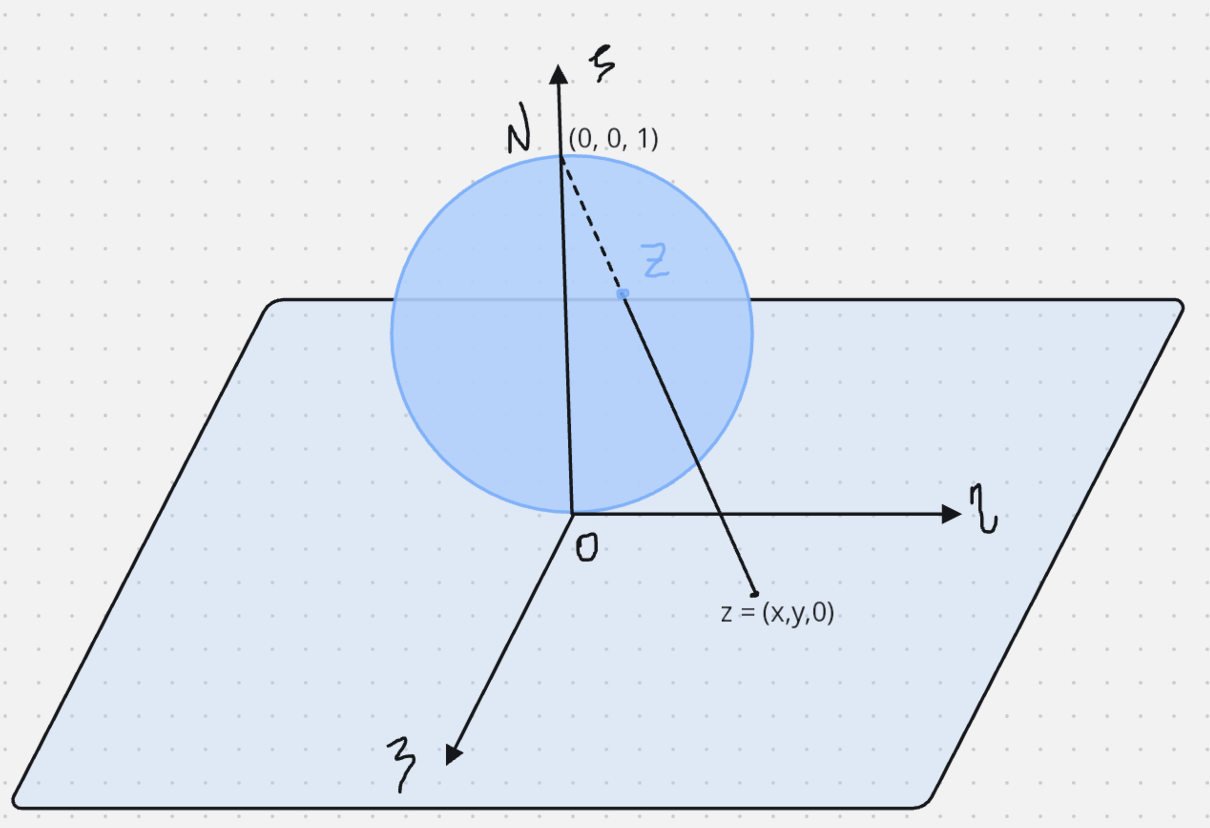
\includegraphics[width=0.6\linewidth]{Riman_sphere.png}
\[\xi^2 + \eta^2 + \left(\zeta - \frac{1}{2}\right)^2 = \frac{1}{4} \text{ -- сфера Римана}\]

\textbfit{Опр.} Стереографической проекцией называется биекция $\mathbb{C}$ и $S \setminus \{N\} : z = (x_0, y_0) \leftrightarrow Z = S \cap zN$
\[N(0, 0, 1) \text{ -- полюс}, \ \overline{a} = (x, y - 1)\]
\[Nz : \begin{cases} \xi = xt \\ \eta = yt \\ \zeta = 1 - t \end{cases}\]
\[x^2t^2 +y^2t^2 + \left(\frac{1}{2} - t\right)^2 = \frac{1}{4}\]
\[t^2(|z|^2+1) = t\]
\[t = \frac{1}{|z|^2+1}\]
\[\begin{cases}
    \xi = \frac{x}{|z|^2+1} \\
    \eta = \frac{y}{|z|^2+1} \\
    \zeta = 1 - \frac{1}{|z|^2+1} = \frac{|z|^2}{|z|^2+1}
\end{cases}\]

Обратно $Z(\xi, \eta, \zeta) \rightarrow z$
\[t = 1 - \zeta, \ x = \frac{\xi}{1-\zeta}, \ y = \frac{\eta}{1-\zeta}\]

\textbfit{Опр.} Говорят, что $z_n \to \infty$, если $|z_n| \to \infty$

\textbfit{Опр.} $\overline{\mathbb{C}} = \mathbb{C} \cup \{\infty\}$ -- расширение комплексной плоскости.

\textbfit{Опр.} Доопределим стереографическую проекцию $\infty \leftrightarrow N$, т.о. это биекция $S$ и $\overline{\mathbb{C}}$.

\textbfit{Опр.} Сферическим расстоянием между $z_1, z_2 \in \overline{\mathbb{C}}$ называется расстояние между их стереографическими проекциями.
\[\rho(z_1, z_2) = |Z_1-Z_2|\]

\textbfit{Утв.} $z_1, z_2 \in \mathbb{C}, \ \rho(z_1, z_2) = \frac{|z_1-z_2|}{\sqrt{1+|z_1|^2}\sqrt{1+|z_2|^2}}, \ \rho(z, \infty) = \frac{1}{\sqrt{1+|z|^2}}$.
\[\triangleright \ \left(\xi, \eta, \zeta\right)\]
\[\rho^2(z_1, z_2) = \left(\frac{x_1}{1+|z_1|^2}-\frac{x_2}{|z_2|^2+1}\right)^2 + \left(\frac{y_1}{1+|z_1|^2} - \frac{y_2}{1+|z_2|^2}\right)^2 + \left(\frac{|z_1|^2}{1+|z_1|^2} - \frac{|z_2|^2}{1+|z_2|^2}\right)^2 =\]
\[=  \ldots = \frac{(x_1-x_2)^2 + (y_1-y_2)^2}{(1+|z_1|^2)(1+|z_2|^2)} \ \blacktriangleleft\]

\textbfit{Утв.} Пусть $|z| \geq R$. Тогда $Z=(\xi, \eta, \zeta) : \zeta \in \left[\frac{R^2}{1+R^2}, 1\right]$.

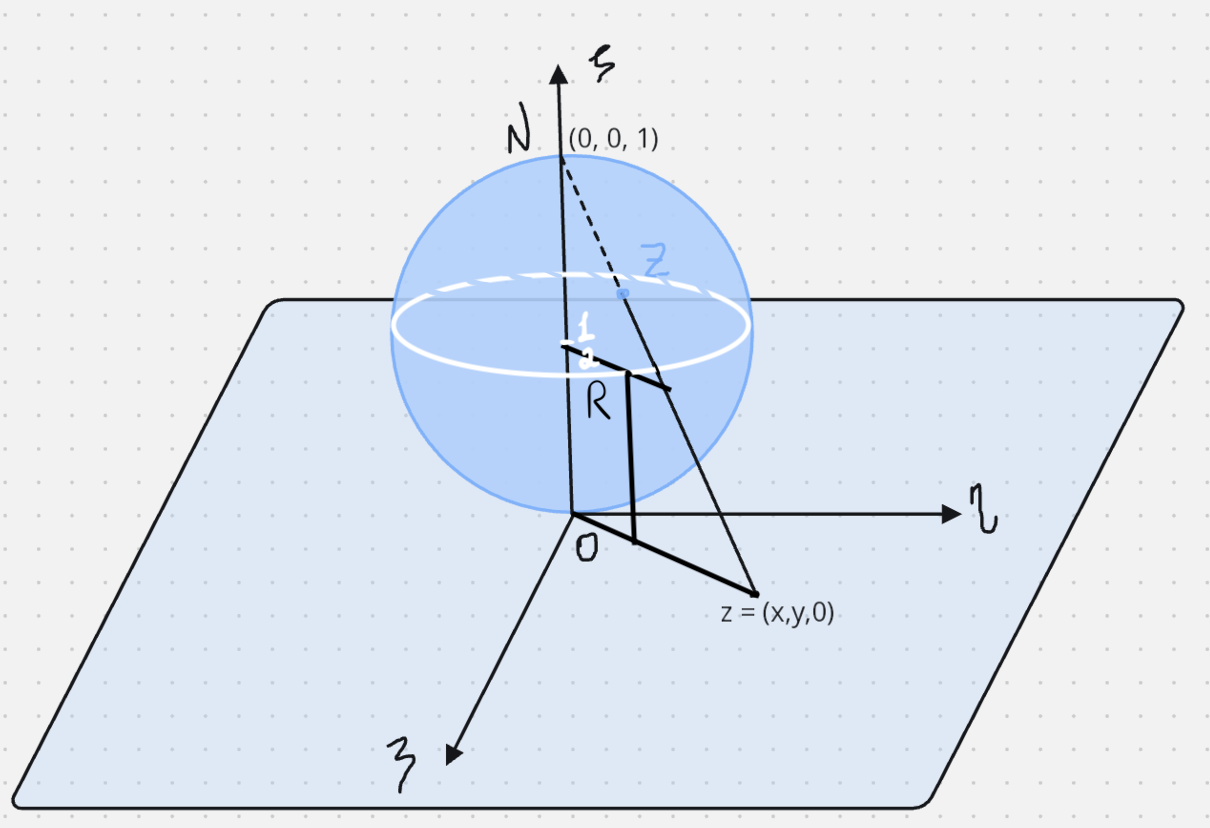
\includegraphics[width=0.6\linewidth]{Riman_sphere_2.png}
\[ \triangleright \ |z| = R\]
\[(\xi, \eta, \zeta) = \left(\frac{x}{|z|^2+1}, \frac{y}{|z|^2+1}, \frac{R^2}{R^2+1}\right)\]
\[\xi^2 + \eta^2 = \frac{x^2+y^2}{(|z|^2+1)^2} = \frac{R^2}{(R^2+1)^2}, \text{ т.е. образ точек такого вида -- окружность } r = \frac{R}{R^2+1}\]
\[\zeta = 1 - \frac{1}{1+R^2} \uparrow |z| \to \infty \ \blacktriangleleft\]
